% !TeX root = RJwrapper.tex
\title{Lending Environment Simulation Model \& Lender Evaluation Tool}
\author{by Vadim Spirkov, Murlidhar Loka}

\maketitle

\abstract{%
Lorem ipsum dolor sit amet, consectetur adipiscing elit. Phasellus
commodo ante risus, sit amet lobortis arcu convallis interdum. Integer
lectus tellus, iaculis sed rhoncus id, eleifend quis purus. Nunc at
tincidunt augue. Curabitur quis odio risus. Nam risus dui, convallis a
hendrerit sit amet, dictum vel felis. (Ref: \cite{combatnoise})
}

% Any extra LaTeX you need in the preamble

\hypertarget{introduction}{%
\section{Introduction}\label{introduction}}

Vestibulum porttitor massa sed ante luctus, interdum ultrices quam
bibendum. Mauris dapibus erat sed ex rutrum tristique. Mauris
condimentum luctus enim, nec lobortis massa auctor a. Maecenas finibus
nibh eget ipsum dictum, sed efficitur turpis mollis. Nulla venenatis,
neque ut commodo pretium, tortor arcu volutpat felis, id condimentum
nulla turpis non nisl. Donec accumsan interdum orci id bibendum.

\begin{Schunk}
\begin{figure}[H]

{\centering 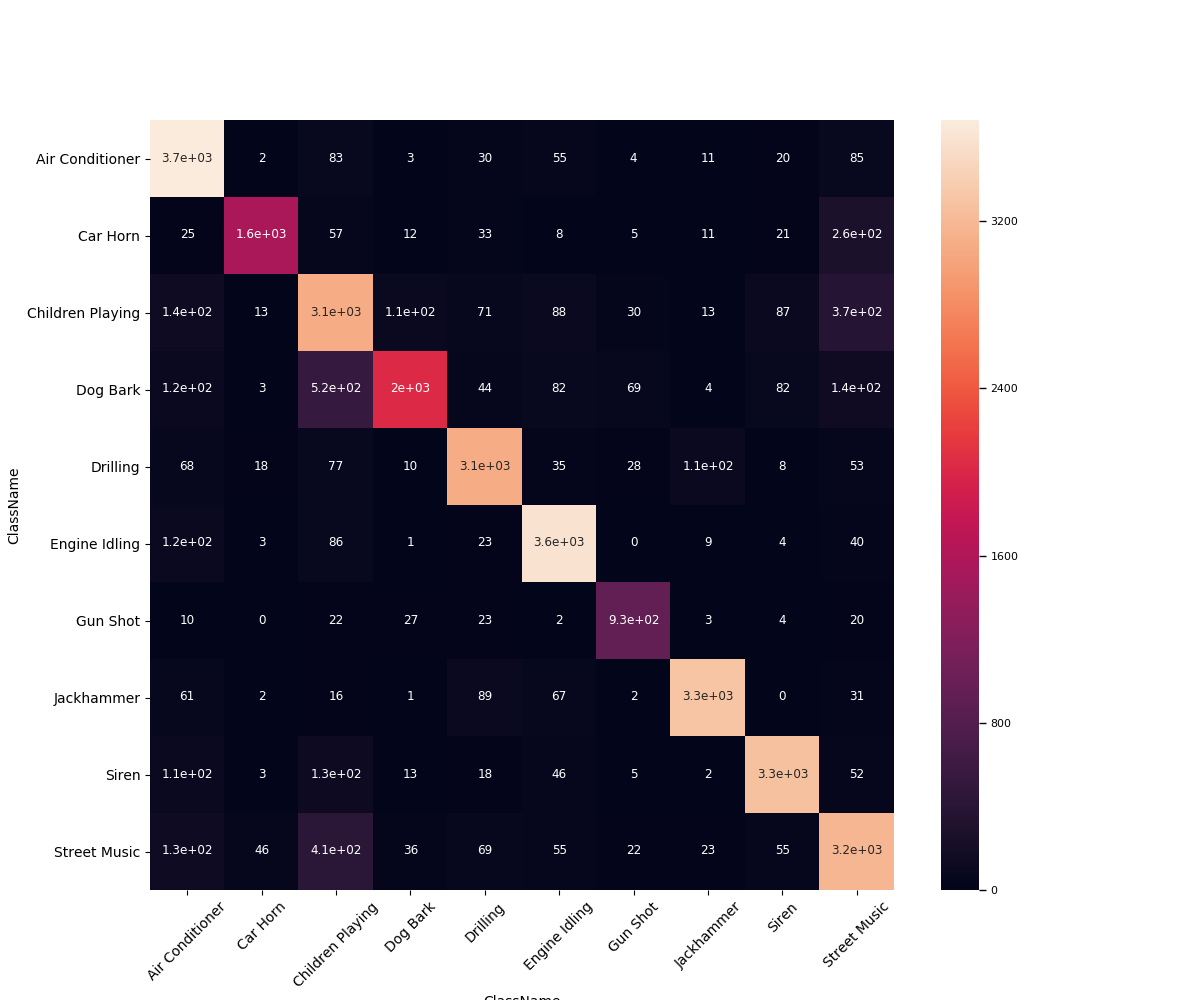
\includegraphics[width=1\linewidth]{../images/test} 

}

\caption[VGG-16 Architecture]{VGG-16 Architecture}\label{fig:example}
\end{figure}
\end{Schunk}

\hypertarget{problem-statement}{%
\section{Problem Statement}\label{problem-statement}}

Vivamus interdum porttitor tellus at lacinia. Duis vitae tempor neque.
Donec vitae pretium justo, ac rutrum neque. Etiam molestie et erat sed
vestibulum. Fusce malesuada, dolor sed pellentesque tincidunt, turpis
neque dignissim orci, ac semper odio neque eu diam. Pellentesque in
purus vitae tortor euismod mollis mollis bibendum neque. Aliquam id nibh
eget velit gravida facilisis. In hac habitasse platea dictumst. Vivamus
sollicitudin metus vel neque consequat, eu rutrum nisi imperdiet. Nunc
scelerisque porta magna et sagittis. Sed et condimentum massa, in
imperdiet est.

\hypertarget{background}{%
\section{Background}\label{background}}

Class aptent taciti sociosqu ad litora torquent per conubia nostra, per
inceptos himenaeos. Nam ultricies, libero sed pulvinar tincidunt, dui
risus volutpat tortor, id viverra purus ligula ut velit. Proin lacinia
tortor purus, a blandit ligula porttitor at. Pellentesque habitant morbi
tristique senectus et netus et malesuada fames ac turpis egestas.

\hypertarget{dataset-description}{%
\section{Dataset Description}\label{dataset-description}}

Sed malesuada eros et augue dignissim, ut consectetur tortor consequat.
Nam sed urna ac lorem finibus aliquam vel sit amet ipsum. Sed ex nulla,
convallis et lectus eu, porta placerat tellus. Nunc gravida est sit amet
tortor elementum auctor. Curabitur justo est, laoreet a sapien ac,
tempor aliquam erat. Proin mattis efficitur nunc a congue. Vivamus
aliquam venenatis augue ac hendrerit. Vestibulum interdum hendrerit
ullamcorper. Cras non imperdiet lacus, consectetur consequat elit. Etiam
non pulvinar elit. Proin egestas egestas nibh, nec facilisis purus
varius id. Nulla facilisi. Mauris sem augue, finibus in nisl vitae,
consectetur ullamcorper enim. Aenean interdum dui sit amet mauris
ultrices, quis facilisis neque aliquet

\begin{verbatim}
              precision    recall  f1-score   support

Air Conditioner    0.83      0.93      0.87      3977
    Car Horn       0.95      0.78      0.86      1998
Children Playing   0.69      0.77      0.73      4009
    Dog Bark       0.91      0.65      0.76      3084
    Drilling       0.89      0.88      0.88      3492
Engine Idling      0.89      0.93      0.91      3877
    Gun Shot       0.85      0.89      0.87      1038
  Jackhammer       0.95      0.92      0.94      3571
       Siren       0.92      0.90      0.91      3656
Street Music       0.75      0.79      0.77      4023

   micro avg       0.85      0.85      0.85     32725
   macro avg       0.86      0.84      0.85     32725
weighted avg       0.85      0.85      0.85     32725
\end{verbatim}

\hypertarget{ml-solution}{%
\section{ML Solution}\label{ml-solution}}

In et est nec ex tincidunt tincidunt in ut dui. Nam vel nulla nec nulla
consectetur sagittis. Vestibulum suscipit sem vitae nisl laoreet tempor.
Suspendisse quis elementum neque. Vivamus dignissim id augue ut laoreet.
Nunc ac tellus tellus. Praesent bibendum eget nisi at accumsan. Quisque
nec ultricies augue. Suspendisse at accumsan est. Duis ac sapien quam.
Sed fermentum in leo non porta. Suspendisse volutpat massa sit amet
vestibulum ornare. Duis ut cursus arcu.

\hypertarget{project-plan}{%
\section{Project Plan}\label{project-plan}}

Suspendisse enim quam, aliquet vel risus ac, elementum egestas ex. Morbi
elit dolor, malesuada posuere ullamcorper volutpat, lobortis quis dui.
Cras nisl quam, finibus vel venenatis a, dapibus vel urna. In hac
habitasse platea dictumst. Quisque scelerisque ante tellus, vel
hendrerit orci vulputate pulvinar. Lorem ipsum dolor sit amet,
consectetur adipiscing elit. Quisque posuere, quam rhoncus faucibus
feugiat, erat tellus dictum nulla, vitae imperdiet dolor turpis non
mauris.

\hypertarget{sub-title-example}{%
\subsection{Sub Title Example}\label{sub-title-example}}

\hypertarget{smaller-title-example}{%
\subsubsection{Smaller title Example}\label{smaller-title-example}}

\bibliography{RJreferences}

\hypertarget{note-from-the-authors}{%
\section{Note from the Authors}\label{note-from-the-authors}}

This file was generated using
\href{https://github.com/rstudio/rticles}{\emph{The R Journal} style
article template}, additional information on how to prepare articles for
submission is here -
\href{https://journal.r-project.org/share/author-guide.pdf}{Instructions
for Authors}. The article itself is an executable R Markdown file that
could be
\href{https://github.com/ivbsoftware/big-data-final-2/blob/master/docs/R_Journal/big-data-final-2/}{downloaded
from Github} with all the necessary artifacts.


\address{%
Vadim Spirkov\\
York University School of Continuing Studies\\
\\
}


\address{%
Murlidhar Loka\\
York University School of Continuing Studies\\
\\
}


